\section{Mathematical Language Processor}\label{sec:mlp}
\glsreset{mlp}\glsreset{pom}\glsreset{bnf}
The \gls{mlp}\footnote{Note that the official publication refers \gls{mlp} to \textit{Mathematical Language \textbf{Processor}}, rather than to the \textbf{parser}. However, the \textit{Mathematical Language Processor} project~\cite{MLP:Project} is slightly different and trying to analyize the natural language context of mathematical expressions. However, both projects are highly coupled and uses the same abbreviation. Since we focus on the parser, we use \gls{mlp} to refer to the \textit{Mathematical Language Parser}, even the official publication understood it as a \textbf{processor}.} project was developed to parse any mathematical expressions~\cite{POM-Tagger}. 

According to \gls{nlp}~\cite{NLP}, the \gls{mlp} understood mathematical expressions as a word of a formal language and parses expressions to so called parse trees. To understand the \gls{mlp}, we need to understand the concept of formal languages first. In the following, we will briefly introduce formal languages~\cite{Math:Encyclopedia:FormalLanguage}.

\begin{definition}[Alphabet]
An \textbf{Alphabet} $\Sigma$ is a finite, non-empty set. The elements of $\Sigma$ are called \textbf{letters} (or \textbf{symbols}).
\end{definition}

For example, the alphabet of a computer is simply the binary alphabet $\Sigma = \{1,0\}$.

\begin{definition}[Word]
A \textbf{word} (or string) $w$ over an alphabet $\Sigma$ is a finite sequence of letters of $\Sigma$. The set of all words over $\Sigma$ is denoted as $\Sigma^\ast$ (known as the Kleene star of $\Sigma$). The empty word $\epsilon$ (sequence of length 0) is always an element of $\Sigma^\ast$.
\end{definition}

\begin{definition}[Formal Language]
A subset $L \subseteq \Sigma^\ast$ is called \textbf{formal language} over an alphabet $\Sigma$.
\end{definition}

Hereafter we use the term \textit{formal language} and \textit{language} interchangeably. Usually, a formal language is constructed by a set of rules. In our case we construct a formal language by a context-free grammar~\cites[79]{Grammar}{IntroComp}.

\begin{definition}[Context-Free Grammar]
A context-free grammar $G = (V, \Sigma, R, S)$ is a $4$-tuple, where
\begin{enumerate}
\item $V$ is a finite set. The elements of $V$ are called \textbf{non-terminal symbols}.
\item $\Sigma$ is a finite set with $\Sigma \cap V = \varnothing$. The elements of $\Sigma$ are called \textbf{terminal symbols}.
\item $R$ is a finite relation from $V$ to $(\Sigma \cup V)^\ast$, thus $R \subseteq V \times (\Sigma \cup V)^\ast$. The members of $R$ are called \textbf{rules}.
\item $S \in V$ is called the \textbf{start symbol}.
\end{enumerate}
\end{definition}

A rule $(\alpha,\beta) \in R$ can be understood as a substitution. We denote the rule also as $\alpha \longrightarrow \beta$.

\begin{definition}[Derived Words \& Applied Rules]
Let $G = (V, \Sigma, R, S)$ be a context-free grammar. Let $A \in V$ and $u,v,w \in (\Sigma \cup V)^\ast$, such that $(A,w) \in R$. Than we say a word '$uwv$' can be \textbf{derived} in one step from the word '$uAv$' by \textbf{applying} the rule $(A,w)$.
\begin{equation}
uAv \Rightarrow uwv.
\end{equation}
\end{definition}

We can also apply multiple rules sequentially. 

\begin{definition}[Chain Derivation]
Let $G = (V, \Sigma, R, S)$ be a context-free grammar and $u,v \in (\Sigma \cup V)^\ast$, with $u \neq v$. We say $v$ can be derived from $u$, if
\begin{equation}
\exists\ k \geq 2\ \ \exists u_1, u_2, \ldots, u_k \in (\Sigma \cup V)^\ast: \quad u = u_1 \Rightarrow u_2 \Rightarrow \ldots \Rightarrow u_k = v,
\end{equation}
and write
\begin{equation}
u \overset{\ast}{\Rightarrow} v.
\end{equation}
\end{definition}

With a context-free grammar, we can define a context-free language over the grammar.

\begin{definition}[Context-Free Language]
Let $G = (V, \Sigma, R, S)$ be a context-free grammar. $G$ defines a language $L(G)$ by
\begin{equation}
L(G) = \left\{ w \in \Sigma^\ast:\ S \overset{\ast}{\Rightarrow} w \right\}.
\end{equation}
\end{definition}

A language $L$ is called \textbf{context-free language} if there is a grammar $G$, such that $L = L(G)$. In other words, a context-free language $L(G)$ is a set of all strings that can be derived from the start variable $S$ of $G$.

\begin{example}\label{ex:cfl}
A simple example for a context-free grammar are well-formed parentheses. Let $V = \{S\},\ \Sigma = \{(,\ )\}$ and $S$ be the start symbol. Furthermore, let $R$ contain the rules
\begin{eqnarray}
&&S \longrightarrow SS\\
&&S \longrightarrow (S)\\
&&S \longrightarrow ()
\end{eqnarray}
Let $G = (V, \Sigma, R, S)$. Than, for example
\begin{equation}\label{eq:example-proof}
\text{'}(()(()))\text{'} \in L(G).
\end{equation}
\end{example}

\begin{proof}[Proof of~\ref{eq:example-proof}]
We can produce the following chain of rules from $R$.
\begin{eqnarray}
S &\Rightarrow & (S)\label{eq:chain}\\
&\Rightarrow & (SS)\notag\\
&\Rightarrow & (()S)\notag\\
&\Rightarrow & (()(S))\notag\\
&\Rightarrow & (()(())).\notag
\end{eqnarray}
Therefore
\begin{equation}
S \overset{\ast}{\Rightarrow} \text{'}(()(()))\text{'} 
\end{equation}
and '$(()(()))$' $\in L(G)$.
\end{proof}

On the other hand
\begin{equation}
\text{'}(()\text{'} \not\in L(G).
\end{equation}

The chain of rules can also be represented in a tree structure. Such trees are called \textbf{parse trees}. The tree for~(\ref{eq:chain}) is visualized in figure~\ref{fig:parseTree}. Note that a parse tree is different to an expression tree. However, a parse tree can become an expression tree if the appropriated mathematical rules are defined.

\begin{figure}[ht]
	\centering
	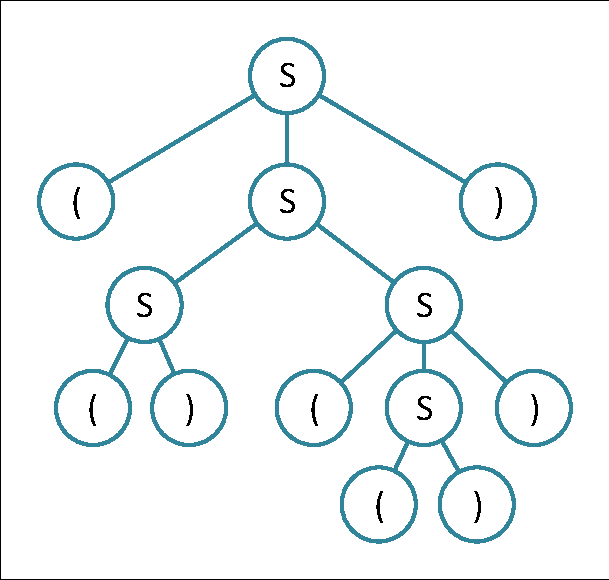
\includegraphics[clip, trim=0.2cm 0.2cm 0.2cm 0.2cm,width=0.6\textwidth]{ParseTree.pdf}
	\caption{The parse tree of the expression '$(()(()))$' for the well-formed parenthesis grammar $G = (V, \Sigma, R, S)$. Produced by the chain of rules~\ref{eq:chain}.}
	\label{fig:parseTree}
\end{figure}

There are several more definitions around formal languages, which we will not mention here. Note, for example, that a parse tree such as in figure~\ref{fig:parseTree} is not necessarily unique and can depend on the choice of a rule where more than one is \textit{applicable}. Consider a context-free grammar for simple arithmetic expressions with sums and subtractions of three variables $x,y$ and $z$. Let $V = \{S\},\ \Sigma = \{x,y,z,+,-\}$, $S$ be the start symbol and define the rules
\begin{eqnarray}
&&S \longrightarrow x\label{eq:chain-1}\\
&&S \longrightarrow y\label{eq:chain-2}\\
&&S \longrightarrow z\label{eq:chain-3}\\
&&S \longrightarrow S + S\label{eq:chain-4}\\
&&S \longrightarrow S - S\label{eq:chain-5}.
\end{eqnarray}
Now an expression such as $x+y-z$ is an element of the context-free language of $G = (V, \Sigma, R, S)$. However, there are two possible parse trees for this expression, tree~\ref{fig:parse1} and \ref{fig:parse2}, depending on the order of which rule gets applied first. Such grammars are also called ambiguous.

\begin{figure}[!ht]
    \centering
    \subfloat[The parse tree of $x+y-z$ if rule~(\ref{eq:chain-4}) gets applied first.]{%
        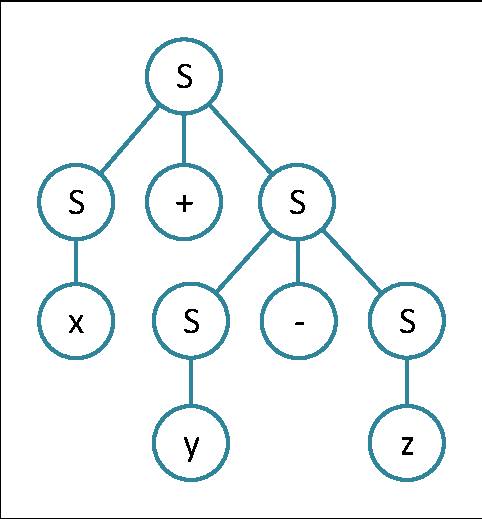
\includegraphics[clip, trim=0.2cm 0.2cm 0.2cm 0.2cm,width=0.4\textwidth]{ParseTree2a.pdf}
        \label{fig:parse1}%
    }
    \hspace{2cm}
    \subfloat[The parse tree of $x+y-z$ if rule~(\ref{eq:chain-5}) gets applied first.]{%
        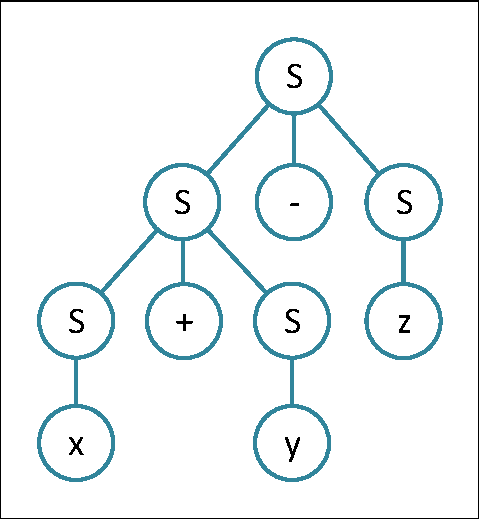
\includegraphics[clip, trim=0.2cm 0.2cm 0.2cm 0.2cm,width=0.4\textwidth]{ParseTree2b.pdf}
        \label{fig:parse2}%
    }
    \caption{Two different parse trees for $x+y-z$. \protect\subref{fig:parse1} applies rule~(\ref{eq:chain-4}) before (\ref{eq:chain-5}), while \protect\subref{fig:parse2} applies the rules vice versa.}
    \label{fig:parseMulti}
\end{figure}

A parser can define now in which order the rules get applied. For example, an \textbf{LL}-Parser parses the input from \textbf{L}eft to right and performing the \textbf{L}eftmost derivations. Leftmost in this terminology means, the parser takes the first applicable rule. In consequence, the internal ordering of rules is no longer irrelevant. The \gls{mlp} is such an \textbf{LL}-Parser. In case of the expression $x+y-z$ from above with the rules~(\ref{eq:chain-1}~-~\ref{eq:chain-5}), an \textbf{LL}-Parser would generates tree~\ref{fig:parse1}.

\subsection{BNF Grammar}
The \gls{bnf} is a notation technique for context-free grammars in computers. For example, a \gls{bnf} specification is a set of rules, written as
\begin{equation}
\verb|<symbol> ::= exp|,
\end{equation}
where \verb|<symbol>| is a non-terminal element and \verb|exp| are one or more sequences of symbols. Symbols that never appear on the left side are terminals.

The \gls{bnf} is often used to describe the syntax of programming languages. There are several tools that automatically generates a parser from a given grammar in \gls{bnf}. One of those tools is \textit{JavaCC} (for Java Compiler Compiler).

\subsection{POM-Tagger \& MLP}\label{subsec:pom-mlp}
The \gls{mlp} defines a \gls{bnf} grammar to parse mathematical \LaTeX{} expressions. The \gls{pom}-tagger (according to Part-of-Speech tagger in \gls{nlp}) categorizes math tokens. The main purpose of the \gls{pom}-tagger is the extraction of semantic information from mathematical \LaTeX. The \gls{pom} tagger is designed to perform multiple \textit{scans}. Given an input \LaTeX{} math document, the first scan of the tagger examines \textit{terms}, and groups them into sub-expressions where suitable. For instance $\verb|\frac{1}{2}|$ consists of two sub-expression of numerator and denominator. A \textit{term} is a non-terminal symbol defined in the \gls{bnf}. In the definition of a \LaTeX{} grammar this can be \LaTeX{} macros, environments, reserved symbols (such as the \LaTeX{} line break command \textbackslash\textbackslash), or numerical or alphanumerical expressions. The first scan of the \gls{pom}-tagger adds information to each term. The information is defined in lexicon files, which provide meanings, descriptions, categories and many more for a large variety of symbols. For example, table~\ref{tab:plus-lex-example} gives an example of the lexicon entry for the plus symbol.

\begin{table}[ht]
	\centering
	\begin{tabular}{lll}
	\hline
	\multicolumn{3}{l}{Symbol: \texttt{+}} \\
	\! & \multicolumn{2}{l}{Feature Set: universal} \\
	\! & \! & Category: operation\\
	\! & \! & Description: plus\\
	\! & \! & Source: unicode-math\\
	\! & \! & \TeX-equivalent: \verb|\mathplus|\\
	\! & \! & Unicode: u+0002b\\
	\hline
	\end{tabular}
	\caption{The lexicon entry for the $+$ symbol.}
	\label{tab:plus-lex-example}
\end{table}

A symbol can be tagged with multiple feature sets according to its ambiguous semantics. Tagged terms are called math terms. Math terms are rarely distinct at this stage and often have multiple features. All information are centralized in the \verb|global-lexicon.txt|.

Further scans will try to reduce the number of alternative feature sets by scanning the context of the math expression and concluding possible feature sets from the structure of the expression. See section~\ref{sec:resolution} for more information about this approach.

In its current state, the \gls{pom}-tagger only performs the first scan. Note that, technically, the \gls{mlp} parses mathematical expressions while the \gls{pom}-tagger categorizes elements of the parse tree. However, the \gls{mlp} also acts as an interface to interact with the parse tree and the \gls{pom}-tagger is a kind of an intermediate step of the whole parsing process. Therefore, we will refer to the \gls{mlp} in following chapters rather than to the \gls{pom}-tagger.

\subsection{MLP-Parse Tree}\label{subsec:mlp-syntax-tree}
Hereafter we consider the \gls{mlp-pt} as the parse tree, which is produced by the \gls{mlp}. The \gls{bnf} of the \gls{mlp} has no mathematical rules implemented in its current state. For example, there is no rule, similar to~(\ref{eq:chain-4}) for the binary operator $+$. Therefore, the \gls{mlp-pt} is not an expression tree. The \gls{pom} project was designed to extract semantic information from mathematical expressions. Certainly, the semantics of mathematical symbols is rarely unique. Consider the $-$ symbol as an example. As a binary operator it indicates the subtraction of two arguments. However, it is also a unary operator as a leading sign.

In its current stage, it is futile to implement arithmetical rules into the \gls{mlp} grammar. The next scan of the \gls{mlp} will reduce ambiguous meanings from the \gls{mlp-pt}. It can be anticipated that the \gls{mlp-pt} will become an expression tree when the planned next scans are implemented.

\begin{figure}[!ht]
    \centering
    \subfloat[The MLP-PT for $a+b$. The POM-Tagger adds information to all terminals. F-Set are feature sets. The terms $a$ and $b$ have multiple feature sets. An F-set represents another semantic meaning. In the figure are not all F-sets listed.]{%
        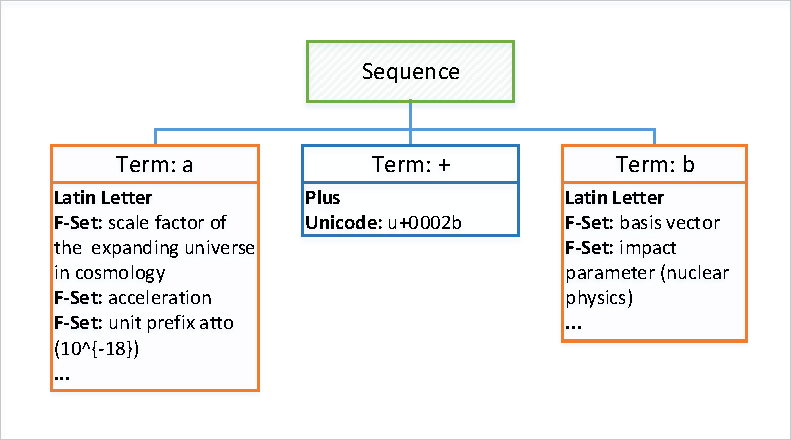
\includegraphics[clip, trim=0.2cm 0.2cm 0.2cm 0.2cm,width=0.65\textwidth]{ParseTreeSimple.pdf}
        \label{fig:tree-parse}%
    }
    \hspace{0.5cm}
    \subfloat[The expression tree for $a+b$.]{%
        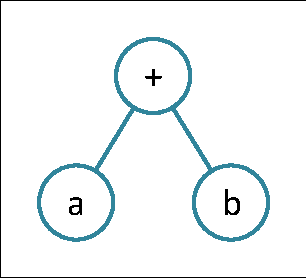
\includegraphics[clip, trim=0.2cm 0.2cm 0.2cm 0.2cm,width=0.25\textwidth]{ExpressionTreeSimple.pdf}
        \label{fig:tree-expr}%
    }
    \caption{Comparing the MLP-Parse tree with an expression tree for $a+b$.}
    \label{fig:tree-compare}
\end{figure}